\section{Utils}

\subsection{Utils}
\begin{frame}[fragile]
\only<1>{
  {\Huge \texttt{snapgauge}}\\
  GUI, Programmiersprache C++, 1500 LOC
}

\only<2>{
\begin{center}
 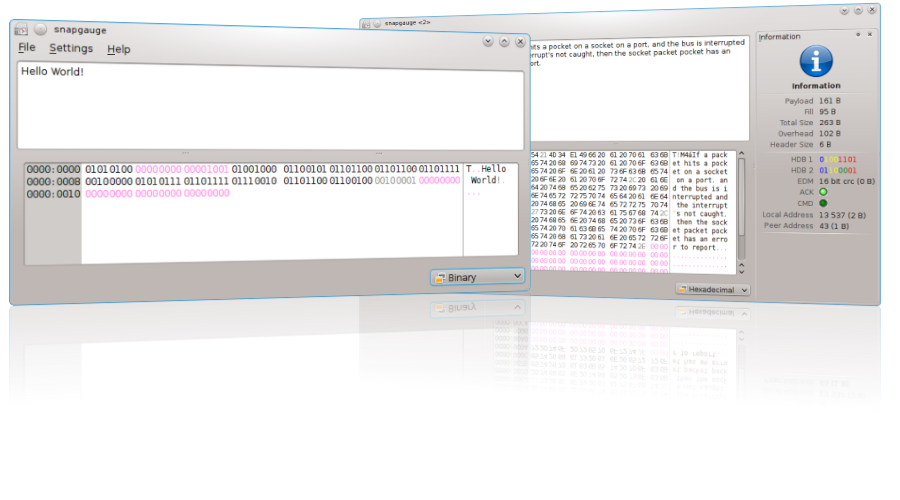
\includegraphics[scale=0.47]{images/screenie_snapgauge.png}
\end{center}
}
\end{frame}

\begin{frame}[fragile]
\begin{center}
 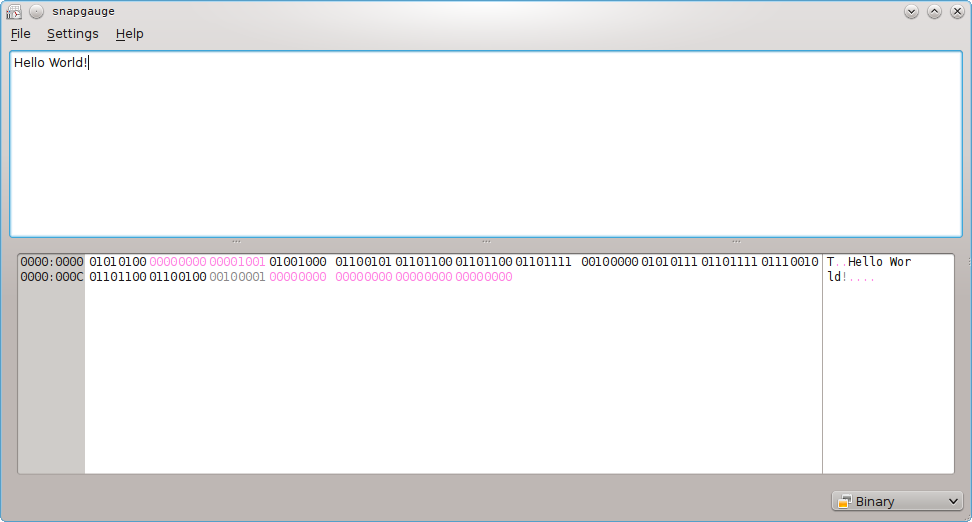
\includegraphics[scale=0.4]{images/snapgauge_1.png}
\end{center}
\end{frame}

\begin{frame}[fragile]
\begin{center}
 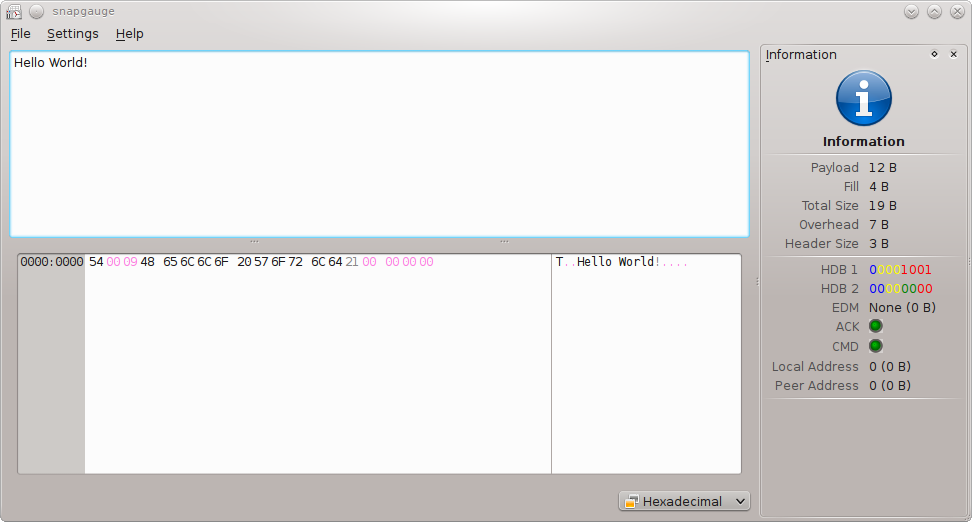
\includegraphics[scale=0.4]{images/snapgauge_2.png}
\end{center}
\end{frame}

\begin{frame}[fragile]
\begin{center}
 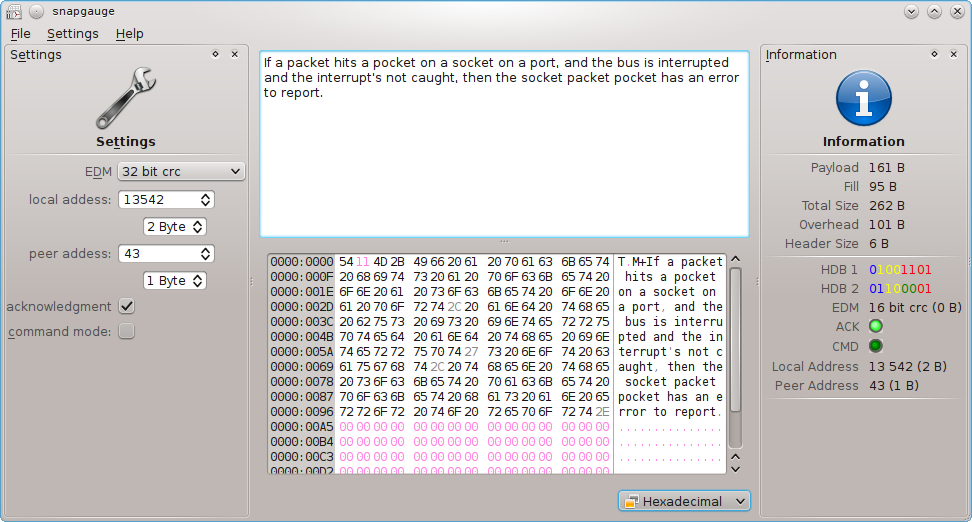
\includegraphics[scale=0.4]{images/snapgauge_3.png}
\end{center}
\end{frame}


% kate: word-wrap off; encoding utf-8; indent-width 4; tab-width 4; line-numbers on; mixed-indent off; remove-trailing-space-save on; replace-tabs-save on; replace-tabs on; space-indent on;
% vim:set spell et sw=4 ts=4 nowrap cino=l1,cs,U1:
